\documentclass[10pt]{report}

\usepackage{graphicx}
\graphicspath{ {./Images/} }
\usepackage{tikz}
\usepackage[T1]{fontenc}
\usepackage{lmodern}
\usepackage{fancyhdr}
\pagestyle{fancy}
\usepackage{caption}
\usepackage{multicol}
\fancyhf{}
\fancypagestyle{plain}{
    \fancyhf{}
    \fancyfoot[C]{\thepage}
    \renewcommand{\headrulewidth}{0pt}
    \renewcommand{\footrulewidth}{0pt}
}
\renewcommand{\headrulewidth}{0pt}
\pagestyle{fancy}
\usepackage[a4paper, top=0in, margin=1in]{geometry}
\fancyfoot[C]{\thepage}
\usepackage{parskip}
\usepackage{hyperref}
\hypersetup{
    colorlinks=true,
    linkcolor=black,
    filecolor=magenta,
    urlcolor=cyan
    }
\usepackage{titlesec}
\usepackage{float}
\usepackage{subfig}

\usepackage[style=ieee]{biblatex}
\addbibresource{references.bib}

\titleformat{\chapter}[display]
  {\normalfont\huge\bfseries}{\chaptertitlename\ \thechapter}{0pt}{\Huge}
\titlespacing*{\chapter}{0pt}{0pt}{10pt}

\newcommand{\includegraphicsrounded}[3]{
    \begin{tikzpicture}
        \clip[rounded corners=1em] (0,0) rectangle node {\includegraphics[width=#2,height=#3]{#1}} (#2,#3);
    \end{tikzpicture}
}

\title{
    \bfseries
    \includegraphicsrounded{figures/birds_of_sweden.png}{12cm}{10cm} \\
    \vspace{1cm}
    \large{Interactive Visualization} \\
    \LARGE{Sweden's vast Bird Fauna} \\
}

\author{
    Nils Fahrni \\
    \small{BSc Data Science Student}
    }
\date{\today}

\begin{document}

\maketitle


\tableofcontents

\chapter{Performance}
\chapter{Design Principles}

\section{Introduction to Shneiderman's Mantra}

In the realm of information visualization, effective data exploration is paramount. Ben Shneiderman, a prominent figure in human-computer interaction, proposed a foundational guideline known as Shneiderman's Mantra to enhance user interaction with complex datasets. The mantra succinctly states: \textit{"Overview first, zoom and filter, then details-on-demand"} \cite{hampdatavisualizationSchneidermansMantra2016}. This principle serves as a blueprint for designing intuitive interfaces that facilitate efficient data analysis.

Shneiderman's Mantra emphasizes a hierarchical approach to data exploration:

\begin{enumerate} \item \textbf{Overview First}: Present the entire dataset in a high-level view to provide context and scope. \item \textbf{Zoom and Filter}: Allow users to focus on subsets of the data that interest them. \item \textbf{Details on Demand}: Enable access to detailed information about specific data points when required. \end{enumerate}

By adhering to this sequence, interfaces can cater to both novice users and experts, providing a scalable means to interact with data of varying complexity.

\section{Implementation in the Birds of Sweden Dashboard}

The Birds of Sweden Dashboard was developed to enable users to navigate and explore Sweden's bird fauna interactively. Implementing Shneiderman's Mantra within this dashboard ensures that users can effectively analyze bird observation data across the country.

\subsection{Overview First}

Upon launching the dashboard, users are presented with a comprehensive map displaying all bird observations across Sweden (Figure~\ref{fig:overview}). This initial view provides an immediate sense of the spatial distribution and density of bird sightings, fulfilling the "Overview First" principle.

\begin{figure}[h] \centering 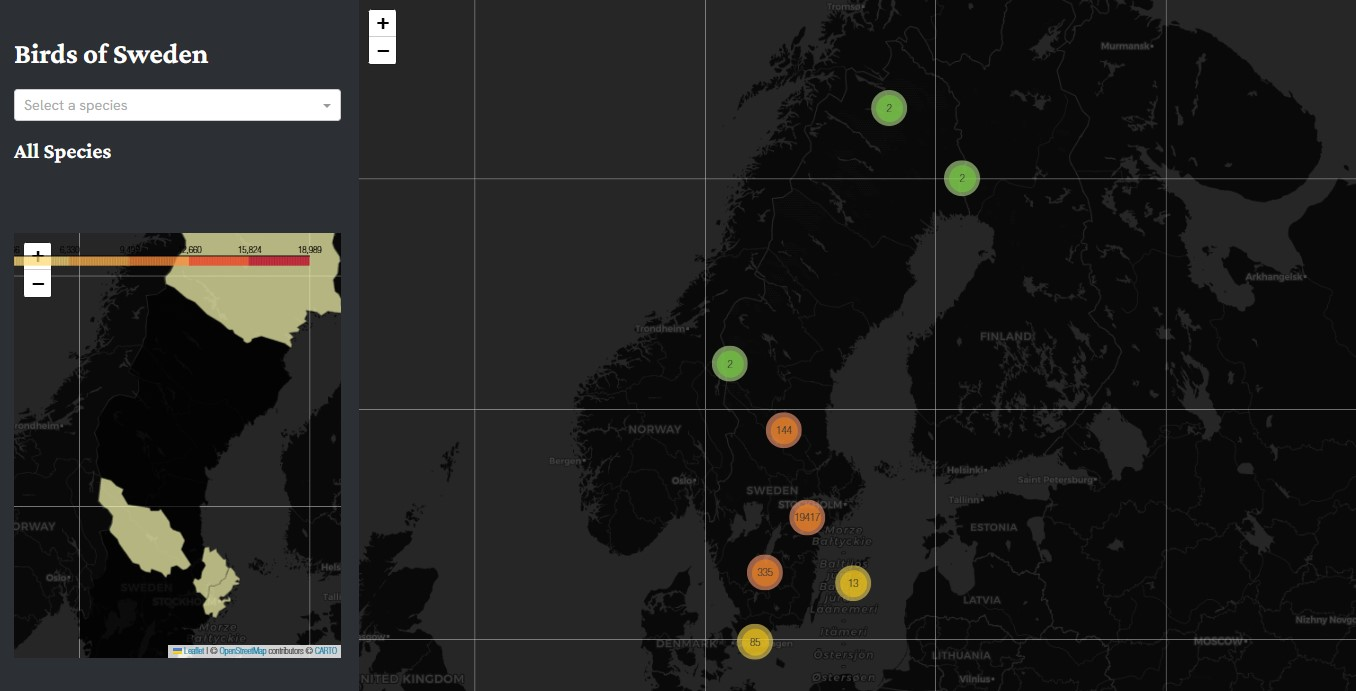
\includegraphics[width=0.8\textwidth]{overview_map.png} \caption{Initial overview of all bird observations in Sweden.} \label{fig:overview} \end{figure}

The map utilizes a scatter plot where each point represents an observation, allowing users to perceive patterns such as hotspots of biodiversity or migratory pathways. Additionally, the sidebar includes a state observations map that consistently displays the entire country's outline, highlighting the number of observations per state. This reinforces the comprehensive nature of the overview.

\subsection{Zoom and Filter}

To facilitate more focused exploration, the dashboard incorporates interactive filtering mechanisms. A dropdown menu enables users to select a specific bird species from an extensive list derived from the dataset (Figure~\ref{fig:dropdown}). Upon selection, the main map updates to display only the observations pertaining to the chosen species.

\begin{figure}[h] \centering 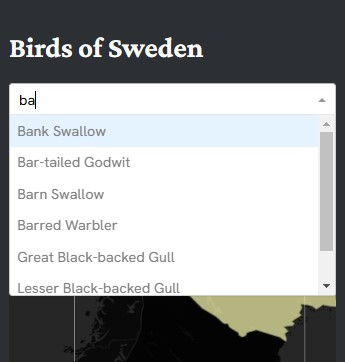
\includegraphics[width=0.4\textwidth]{species_dropdown.png} \caption{Species selection dropdown for filtering observations.} \label{fig:dropdown} \end{figure}

This filtering capability exemplifies the "Zoom and Filter" principle, allowing users to narrow down the dataset to areas or species of interest. The state observations map in the sidebar also updates accordingly, highlighting only the states where the selected species has been observed, thus providing a filtered geographical context (Figure~\ref{fig:filtered_map}).

\begin{figure}[h] \centering \includegraphics[width=0.8\textwidth]{filtered_map.png} \caption{Map displaying observations of a selected species after filtering.} \label{fig:filtered_map} \end{figure}

\subsection{Details on Demand}

To offer in-depth information, the dashboard provides detailed data about specific observations and species. When a species is selected, the sidebar displays:

\begin{itemize} \item \textbf{Species Name and Scientific Name}: Clarifies the common and scientific nomenclature. \item \textbf{Species Image}: Retrieves an image from Wikipedia for visual identification. \item \textbf{Additional Information}: Presents taxonomic order, observation count, breeding category, state, and locality. \end{itemize}

This implementation of "Details on Demand" ensures that users can access specific information without overwhelming the initial view. Moreover, clicking on an observation point on the map sets the species in the dropdown, updating the sidebar with relevant details (Figure~\ref{fig:details_on_demand}).

\begin{figure}[h] \centering 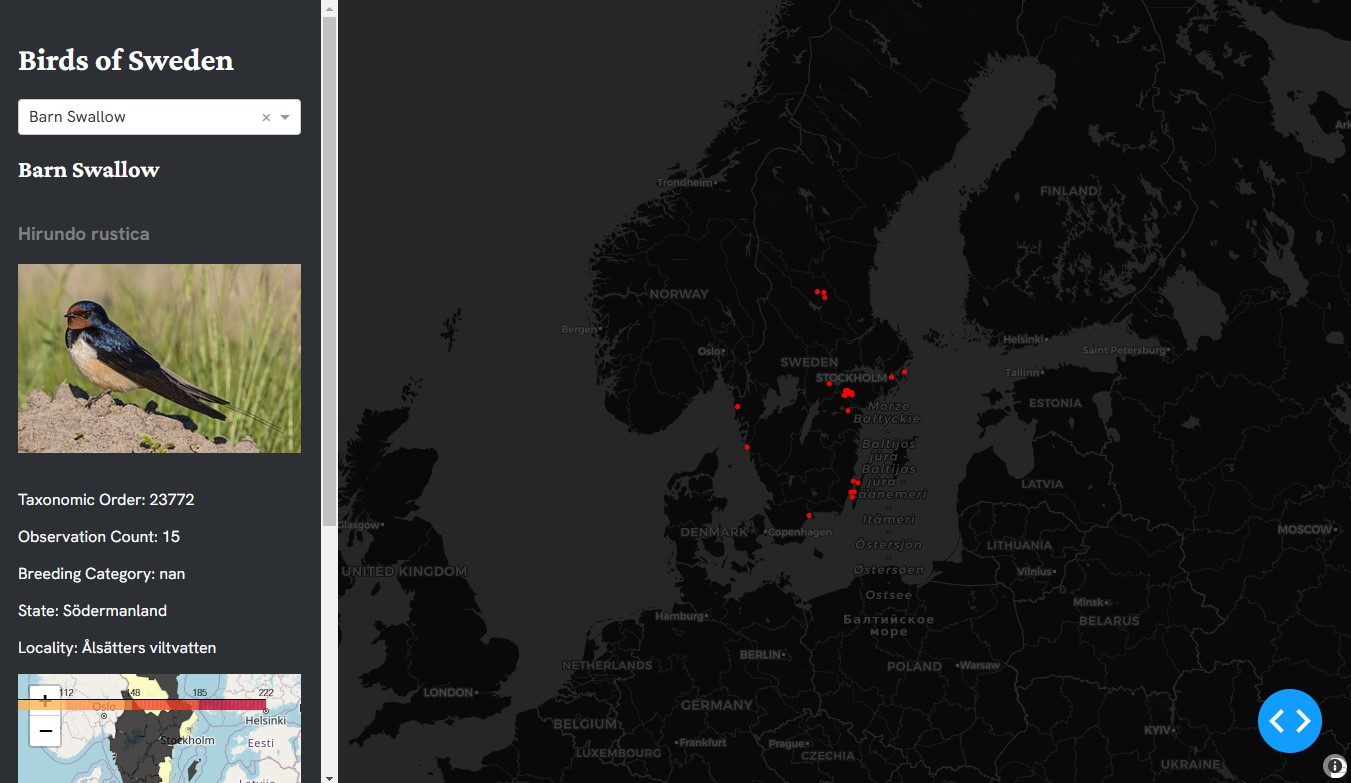
\includegraphics[width=0.4\textwidth]{species_details.png} \caption{Detailed information displayed upon species selection.} \label{fig:details_on_demand} \end{figure}

\subsection{Technical Implementation}

The dashboard leverages the Dash framework for Python, enabling the creation of interactive web applications. Key implementation aspects include:

\begin{itemize} \item \textbf{Data Loading}: The full dataset is loaded without slicing to ensure all observations and species are available. \item \textbf{Data Cleaning}: Missing values in critical columns such as \texttt{LATITUDE}, \texttt{LONGITUDE}, and \texttt{COMMON NAME} are handled to prevent empty maps or dropdowns. \item \textbf{Callbacks}: Dash callbacks are used to update the map and sidebar components dynamically based on user interactions. \item \textbf{Geographical Consistency}: The state observations map uses the \texttt{fitbounds="geojson"} parameter to always display the entire country's outline, regardless of the data filtered. \end{itemize}

By addressing initial issues such as empty maps on startup and mismatches in state naming conventions, the dashboard now aligns with the intended functionality and provides a seamless user experience.

\section{Goals and Hopes for the Dashboard}

The primary objective of implementing Shneiderman's Mantra in the Birds of Sweden Dashboard is to enhance user interaction and facilitate the exploration of bird fauna data. The specific goals include:

\subsection{Improving User Interaction and Experience}

By providing an intuitive interface that adheres to established principles of information visualization, users can navigate the dataset effectively, regardless of their familiarity with the data. The hierarchical approach reduces cognitive load and allows for a more engaging experience.

\subsection{Facilitating Exploration of Sweden's Bird Fauna}

The dashboard serves as an educational tool, enabling users to discover patterns and insights within the bird observation data. For instance, users can identify regions with high biodiversity, track migration patterns, or explore species distribution.

\subsection{Enabling Users to Gain Insights}

Through interactive filtering and detailed information access, users can perform analyses that may lead to new findings or support research efforts. Conservationists, ornithologists, and bird enthusiasts alike can leverage the dashboard to inform their work or interests.

\section{Conclusion}

Implementing Shneiderman's Mantra in the Birds of Sweden Dashboard has resulted in a powerful tool for data exploration. By providing an initial overview, enabling focused filtering, and offering detailed information on demand, the dashboard aligns with best practices in information visualization. The hope is that this approach not only enhances user engagement but also contributes to a deeper understanding of Sweden's rich bird fauna.
\chapter{HCI Basics}
\chapter{Evaluation}

Evaluating the usability and user experience of an interactive visualization is crucial to ensure it meets the needs of its intended audience. This chapter presents an evaluation of the \textit{Birds of Sweden Dashboard} through a qualitative user study involving five participants from a range of backgrounds. The goal is to gain insights into how different users perceive and interact with the dashboard, identifying strengths and areas for improvement.

\section{Methodology}

\subsection{Selection of Evaluation Method}

A qualitative interview approach was chosen for this evaluation due to its effectiveness in exploring users' thoughts, feelings, and experiences in depth. Unlike quantitative methods, qualitative interviews allow for open-ended responses, providing rich insights into user behavior and preferences. This method is appropriate for measuring user experience in the context of the dashboard, as it enables the identification of usability issues and the collection of detailed feedback that can inform future design enhancements.

\subsection{Participants}

Five users with varying backgrounds, expertise, and interests related to bird observation and data visualization were involved in a qualitative interview:

\begin{enumerate} 
    \item \textbf{Participant 1} -- A 31-year-old bird enthusiast and amateur photographer who enjoys birdwatching during her travels across Sweden.
    \item \textbf{Participant 2} -- A 50-year-old conservationist and hobby ornotihologist.
    \item \textbf{Participant 3} -- A 23-year-old web developer studying Data Science.
    \item \textbf{Participant 4} -- A 24-year-old carpenter, now studying Data Science.
    \item \textbf{Participant 5} -- A 65-year-old retiree who recently started birdwatching as a hobby and is not very tech-savvy.
\end{enumerate}

\section{Interview Questions}

Five open-ended questions were designed to explore key aspects of the user experience:

\begin{enumerate}
    \item \textbf{How intuitive did you find the navigation and interaction with the dashboard?}

    \textit{Purpose}: To assess the overall usability and whether users can navigate the interface without confusion.

    \item \textbf{What features did you find most useful or engaging, and why?}

    \textit{Purpose}: To identify which elements of the dashboard are most valued by users, informing future enhancements.

    \item \textbf{Were there any difficulties or frustrations you encountered while using the dashboard?}

    \textit{Purpose}: To uncover usability issues or pain points that need to be addressed.

    \item \textbf{How well does the dashboard cater to your specific needs or interests related to bird observation?}

    \textit{Purpose}: To evaluate the dashboard's effectiveness in meeting the diverse needs of different user groups.

    \item \textbf{What improvements or additional features would you suggest for the dashboard?}

    \textit{Purpose}: To gather user-driven ideas for enhancements that could improve satisfaction and usability.
\end{enumerate}

\section{Results}

The participants' responses are summarized below. Tables are used to present the key points from each interview for clarity.

\begin{table}[H]
    \centering
    \begin{tabular}{p{3cm} | p{12cm}}
        \hline
        \textbf{Participant} & \textbf{Responses} \\
        \hline
        \multicolumn{2}{l}{\textbf{Question 1: Navigation and Interaction Intuitiveness}} \\
        \hline
        Participant 1 & Found the dashboard mostly intuitive. Initially unsure about how to interact with map points but appreciated the straightforward species selection once she became accustomed. \\
        \hline
        Participant 2 & Navigated easily due to familiarity with similar tools; praised the clean, professional interface but noted the potential for advanced navigational aids for detailed searches. \\
        \hline
        Participant 3 & Found the interface user-friendly and intuitive, commended the responsive design, though noted minor inconsistencies in menu transitions. \\
        \hline
        Participant 4 & Experienced slight confusion with sidebar updates not being immediately noticeable; suggested clearer visual cues for when data changes. \\
        \hline
        Participant 5 & Initially overwhelmed but adapted quickly after a brief exploration. Appreciated the clear dropdown menu once located but felt it could be made more visible. \\
        \hline
        \multicolumn{2}{l}{\textbf{Question 2: Most Useful or Engaging Features}} \\
        \hline
        Participant 1 & Enjoyed the species images and detailed descriptions, particularly appreciating the ability to locate her favorite birds' habitats. \\
        \hline
        Participant 2 & Valued the observation distribution visualizations, which were highly useful for understanding migration patterns. \\
        \hline
        Participant 3 & Was particularly impressed by the interactive maps and their hover effects, which dynamically updated related data. \\
        \hline
        Participant 4 & Found the state-level observation map valuable for identifying regions that might require conservation efforts. \\
        \hline
        Participant 5 & Loved the ability to explore species and their habitats through the interactive maps, finding the feature highly educational and engaging. \\
        \hline
    \end{tabular}
    \caption{Participant Responses to Questions 1 and 2}
    \label{tab:responses1}
\end{table}


\begin{table}[H]
    \centering
    \begin{tabular}{p{3cm} | p{12cm}}
        \hline
        \textbf{Participant} & \textbf{Responses} \\
        \hline
        \multicolumn{2}{l}{\textbf{Question 3: Difficulties or Frustrations}} \\
        \hline
        Participant 1 & Struggled to hover over small map points; suggested larger clickable areas or a zoom-in feature to make interactions easier. \\
        \hline
        Participant 2 & Felt the lack of advanced filtering options (e.g., by date range or observation count) limited deeper analyses. \\
        \hline
        Participant 3 & Noted issues with mobile responsiveness, particularly on tablets where some menu elements were misaligned. \\
        \hline
        Participant 4 & Encountered challenges when using assistive technology; highlighted the importance of improving accessibility features. \\
        \hline
        Participant 5 & Was initially confused about the species selection due to the dropdown’s placement and size but adapted after finding it. \\
        \hline
        \multicolumn{2}{l}{\textbf{Question 4: Catering to Specific Needs or Interests}} \\
        \hline
        Participant 1 & Found the dashboard catered well to her interest in discovering new birdwatching spots and learning about bird habitats. \\
        \hline
        Participant 2 & Appreciated the geographical data but desired more detailed analytics and tools to support academic research needs. \\
        \hline
        Participant 3 & Found the dashboard inspiring for his studies in design and praised its application of interaction design principles. \\
        \hline
        Participant 4 & Saw potential for using the dashboard in conservation planning but wanted more data layers, such as vegetation and climate overlays. \\
        \hline
        Participant 5 & Enjoyed learning about bird species and habitats, which added excitement to her beginner birdwatching efforts. \\
        \hline
        \multicolumn{2}{l}{\textbf{Question 5: Suggestions for Improvement}} \\
        \hline
        Participant 1 & Suggested adding bird call sounds for a richer experience and a tutorial to guide new users through the dashboard. \\
        \hline
        Participant 2 & Recommended incorporating time-series data to observe seasonal trends and changes in bird populations over the years. \\
        \hline
        Participant 3 & Proposed improving mobile responsiveness and adding gesture controls to enhance usability on touchscreens. \\
        \hline
        Participant 4 & Highlighted the need for accessibility features like screen reader support, high-contrast modes, and keyboard navigation. \\
        \hline
        Participant 5 & Suggested simplifying the interface with larger text and icons to make it more beginner-friendly and accessible. \\
        \hline
    \end{tabular}
    \caption{Participant Responses to Questions 3, 4, and 5}
    \label{tab:responses2}
\end{table}


\section{Analysis}

The qualitative interviews revealed several key themes and insights:

\subsection{Usability and Navigation}

Most participants found the dashboard intuitive, particularly those with technical backgrounds. However, less tech-savvy users like Sara experienced initial confusion, indicating a need for improved onboarding or tutorials. The visibility of interactive elements like the species dropdown could be enhanced to aid navigation.

\subsection{Engaging Features}

Interactive maps and species information were consistently highlighted as valuable features. Visual representations and the inclusion of images contributed positively to user engagement, aligning with the importance of visual elements in interaction design.

\subsection{Usability Issues and Frustrations}

Common difficulties included:

\begin{itemize}
    \item \textbf{Hovering over Data Points}: Small interactive areas made it challenging to access tooltips, supporting the need to apply Fitts's Law considerations.
    \item \textbf{Accessibility}: Users like Olle emphasized the lack of support for assistive technologies, echoing the findings from the literature on accessible visualization.
    \item \textbf{Mobile Optimization}: Issues on tablets and mobile devices suggest the dashboard is not fully responsive, limiting usability across devices.
\end{itemize}

\subsection{Meeting User Needs}

Participants with specific interests, such as conservation and research, found the dashboard partially met their needs but desired more advanced features like filtering options and additional data layers. This indicates opportunities to expand functionality to cater to specialized user groups.

\subsection{Suggestions for Improvement}

Key recommendations included:

\begin{itemize}
    \item \textbf{Enhancing Accessibility}: Implementing features like screen reader support and high-contrast modes.
    \item \textbf{Mobile Responsiveness}: Optimizing the dashboard for use on tablets and smartphones.
    \item \textbf{Interactive Enhancements}: Adding bird sounds, gesture controls, and tutorials to improve engagement and usability.
    \item \textbf{Advanced Features}: Incorporating time-series data and advanced filtering to support research and conservation efforts.
\end{itemize}

\printbibliography

\end{document}